\documentclass{beamer}
%
% Choose how your presentation looks.
%
% For more themes, color themes and font themes, see:
% http://deic.uab.es/~iblanes/beamer_gallery/index_by_theme.html
%
\mode<presentation>
{
  \usetheme{Madrid}      % or try Darmstadt, Madrid, Warsaw, ...
  \usecolortheme{beaver} % or try albatross, beaver, crane, ...
  \usefonttheme{serif}  % or try serif, structurebold, ...
  \setbeamertemplate{navigation symbols}{}
  \setbeamertemplate{caption}[numbered]
} 

\usepackage{hyperref}
\usepackage[english]{babel}
\usepackage[utf8x]{inputenc}
\usepackage{pdfpages}
\usepackage{framed, color}
\definecolor{shadecolor}{rgb}{1,0.8,0.3}
\usepackage{color}
 
\definecolor{codegreen}{rgb}{0,0.6,0}
\definecolor{codegray}{rgb}{0.5,0.5,0.5}
\definecolor{codepurple}{rgb}{0.58,0,0.82}
\definecolor{backcolour}{rgb}{0.95,0.95,0.92}
\definecolor{pblue}{rgb}{0.13,0.13,1}
\definecolor{pgreen}{rgb}{0,0.5,0}
\definecolor{pred}{rgb}{0.9,0,0}
\definecolor{pgrey}{rgb}{0.46,0.45,0.48}
 
\usepackage{listings}
\lstset{language=Python,
  showspaces=false,
  showtabs=false,
  breaklines=true,
  showstringspaces=false,
  breakatwhitespace=true,
  commentstyle=\color{pgreen},
  keywordstyle=\color{pblue},
  stringstyle=\color{pred},
  basicstyle=\ttfamily,
  frame=lrbt,xleftmargin=\fboxsep,xrightmargin=-\fboxsep
}

\title[Ragazze Digitali 2019]{Ragazze Digitali A.A. 2018/2019}
\author{E. Salvucci - S. Gattucci - C. Varini}
\date{}

\AtBeginSection[]
{
  \begin{frame}<beamer>
    \frametitle{Outline}
    \tableofcontents[currentsection,currentsubsection]
  \end{frame}
}

\begin{document}

\setbeamertemplate{background}
{
\includegraphics[width=\paperwidth,height=\paperheight]{images/ragazze_digitali.jpg}}
\begin{frame}
\end{frame}

\setbeamertemplate{background}
% Python

\begin{frame}{Cosa faremo oggi}
    \vspace{0.8cm}
      Costruiremo un programma che sarà in grado di convertire un normale testo in un codice segreto e viceversa.
\end{frame}

\begin{frame}{Caesar Chiper}
    Vuoi criptare o decriptare un messaggio?\newline
    \textbf{ciptare}\newline
    Scrivi il tuo messaggio:\newline
    \textbf{Questo è il corso Ragazze digitali, idee per un futuro smart}\newline
    Inserisci la chiave (1-52)\newline
    \textbf{13}\newline
    Ecco il testo criptato:\newline
    dHrFGB zèz zvy zpBEFB zentnMMr zqvtvGnyv,z zvqrr zCrE zHA zsHGHEB zFznEG
\end{frame}

\section{Crittografia}

\begin{frame}[fragile]
\frametitle{Crittografia 1/3}
Vediamo di imparare qualche nozione elementare di crittografia che ci può essere utile per scrivere il nostro programma
\begin{block}{Per iniziare}
	\begin{itemize}
		\item \textbf{chiper} = è il sistema, l'insieme delle regole secondo le quali \textit{criptiamo} un messaggio
		\item \textbf{plaintext} = testo che vogliamo nascondere e mantenere segreto
		\item \textbf{chipertext} = testo trasformato
		\item un \textit{plaintext} viene \textbf{criptato} in un \textit{chipertext}
		\item un \textit{chipertext} viene \textbf{decriptato} in un \textit{plaintext}
		\item \textbf{chiave} = valore segreto con il quale si decripta un messaggio criptato usando un determinato \textbf{chiper}
	\end{itemize}
\end{block}
    
\end{frame}

\begin{frame}[fragile]
\frametitle{Crittografia 2/3}
Esistono tantissimi chiper, sistemi per crittografare un messaggio, ciascuno con la propria chiave. Per costruire il nostro programma ci interesseremo del \textbf{Caeser chiper}, ovvero del \textit{cifrario di Cesare}.. Si, proprio quel Cesare che pensate! ...E' parecchio vecchio come chiper, ma tutt'ora ancora perfettamente funzionante.

\end{frame}

\begin{frame}[fragile]
\frametitle{Crittografia 3/3}

\begin{columns}[T]
	\begin{column}[T]{0.6\textwidth}
		Con questo Caeser chiper, i messaggi vengono criptati rimpiazzando ciascuna lettera con una lettera \textit{"shiftata"}, ovvero spostata.\newline
		Per esempio, se \textit{shiftiamo} di 3 lettere, avremo che la lettera \textbf{B} diventerà una \textbf{E}, e così via. Per decriptare i messaggi, verranno shiftate indietro le lettere e quindi una \textbf{E} diventerà una \textbf{B}.	
	\end{column}
	\begin{column}[T]{0.4\textwidth}
		\begin{figure}[t]
			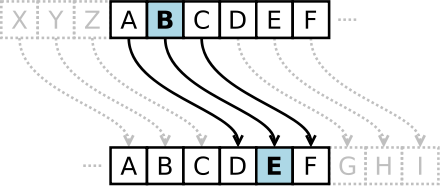
\includegraphics[height=2.7cm, width=\textwidth]{images/Caesar.png}
		\end{figure}
	\end{column}
\end{columns}
\begin{figure}[t]
	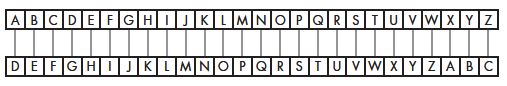
\includegraphics[height=2.5cm, width=\textwidth]{images/AlfabetoCaeser.png}
\end{figure}
La \textbf{chiave} del Caeser chiper è il numero di lettere shiftate.
\end{frame}

\setbeamertemplate{background}{}

\section{Metodo find() delle stringhe}

\begin{frame}[fragile]
\frametitle{string.find()}
\begin{block}{Come funziona}
	\begin{itemize}
		\item E' un metodo che restituisce la posizione in cui si trova la stringa passata al metodo rispetto alla stringa su cui è invocato il metodo.
		\item Proviamo a vedere con degli esempi come funziona
	\end{itemize}
\end{block}
\begin{columns}
	\begin{column}[T]{0.53\textwidth}
		\begin{lstlisting}
>'Hello world'.find('H')
0
>'Hello world'.find('o')
4
>'Hello world'.find('ell')
1
>'Hello world'.find('xyz')
-1
		\end{lstlisting}
	\end{column}
	\begin{column}[T]{0.47\textwidth}
		\begin{itemize}
			\item La numerazione degli indici parte da 0 e non da 1!
			\item Di 'o' ce ne sono due, ma viene restituito l'indice della prima occorrenza trovata
			\item Se si ricerca una stringa, viene restituito l'indice dell'inizio della stringa
			\item Se si cerca una stringa non presente, viene restituito -1
		\end{itemize}
	\end{column}
\end{columns}

\end{frame}

\section{Metodo len()}

\begin{frame}[fragile]
\frametitle{len()}
\begin{block}{Come funziona}
	\begin{itemize}
		\item E' un metodo che restituisce il numero di caratteri presenti nella stringa passata in input
		\item Proviamo a vedere con degli esempi come funziona
	\end{itemize}

	\begin{lstlisting}
SYMBOLS = 'ABCDEFGHIJKLMNOPQRSTUVWXYZ'
MAX_KEY_SIZE = len(SYMBOLS)
	\end{lstlisting}	
	\begin{itemize}
		\item In questo esempio, la variabile globale \texttt{SYMBOLS} contiene una stringa rappresentante tutte le lettere dell'alfabeto.
		\item La variabile globale \texttt{MAX\_KEY\_SIZE}, invece, contiene il risultato della chiamata alla funzione \textbf{len()} invocata con parametro la stringa di cui vogliamo calcolare la lunghezza
	\end{itemize}
\end{block}
\end{frame}

\section{Caeser chiper}

\begin{frame}[fragile]
\frametitle{Caeser chiper 1/5}
\begin{block}{Ora tocca a voi!}
	\begin{itemize}
		\item Definisci innanzitutto due variabili globali, una contenente tutte le lettere dell'alfabeto (minuscole e maiuscole) e un'altra che contenga il numero delle lettere definite in precedenza
		\item Costruisci una funzione che chieda all'utente se vuole criptare o decriptare un messaggio e che restituisca la modalità scelta dall'utente; altrimenti, se l'utente inserisce un carattere o una stringa non inerente alla scelta, viene mostrato un messaggio di spiegazione su cosa bisogna inserire e viene riproposta la domanda iniziale.
		\item \textbf{Suggerimento}: per controllare cosa inserisce l'utente, può essere di aiuto convertire l'input in caratteri \textit{lowercase} 
	\end{itemize}
\end{block}
\end{frame}

\begin{frame}[fragile]
\frametitle{Caeser chiper 2/5}
\begin{block}{Ora tocca a voi!}
	\begin{itemize}
		\item Costruisci una funzione che chieda all'utente di inserire il messaggio che vuole criptare/decriptare e lo restituisca come valore di ritorno della funzione.
		\item Costruisci una funzione che chieda all'utente di inserire la chiave di cifratura, che sarà un numero compreso tra 1 e il numero delle lettere definite all'inizio. Controllare che il valore inserito sia all'interno di questo range. Nel caso non lo fosse, deve essere richiesto all'utente di inserire la chiave; se è dentro al range, viene restituito dalla funzione.
	\end{itemize}
\end{block}
\end{frame}

\begin{frame}[fragile]
\frametitle{Caeser chiper 3/5}
\begin{block}{Ora tocca a voi!}
	\begin{itemize}
		\item Costruisci una funzione che effettivamente cripta o decripta il messaggio in base a cosa è stato scelto dall'utente e alla chiave scelta. 
		\item Per ogni simbolo (carattere) del nostro messaggio, se il carattere è presente nella nostra lista caratteri (ovvero vuol dire che appartiene all'alfabeto), dobbiamo salvarci l'indice del nuovo carattere da sostituire, in base alla chiave scelta.
		\item Una volta trovato il nuovo indice, creiamo un array con la nuova stringa, inserendo carattere per carattere. Infine si restituisca l'array.
		\item Se il carattere non è presente nella nostra lista, copiamo semplicemente il vecchio carattere senza sostituirlo.
	\end{itemize}
\end{block}
\end{frame}

\begin{frame}[fragile]
\frametitle{Caeser chiper 4/5}
\begin{block}{Ora tocca a voi!}
	\begin{itemize}
		\item In questa ultima funzione per prima cosa bisogna verificare se è stata scelta la modalità decriptazione: con essa, infatti, è necessario rendere negativa la chiave, così che nella fase di sostituzione del carattere esso venga sostituito con il corrispettivo simbolo.
		\item Inseriamo quindi questo pezzetto di codice:
	\end{itemize}
\end{block}
\begin{lstlisting}
if mode[0] == 'd':
    key = -key
translated = '' # inizializziamo a nullo il vettore che conterra' la stringa finale
\end{lstlisting}
\end{frame}

\begin{frame}[fragile]
\frametitle{Caeser chiper 5/5}
\begin{block}{Ora tocca a voi!}
	\begin{itemize}
		\item Come ultima cosa richiamate le funzioni, salvate i valori restituiti e stampate la stringa criptata o decriptata!
		\item Ed ecco, il nostro cifrario è completato! 
	\end{itemize}
\end{block}

\end{frame}
\end{document}